\section{Programação do sistema} % ### 5.5.1. História do desenvolvimento

%% Acho que vai ficar mais fácil assim

% considerando que é uma das mais utilizadas no mercado para desenvolvimento web [buscar referência]

Após a elaboração dos protótipos com o Figma, e da conceitualização diagramática do banco de dados, o desenvolvimento do sistema foi iniciado. Por maior familiaridade com a linguagem foi escolhida a linguagem JavaScript, utilizando a biblioteca \textit{React} para a criação dos componentes visuais, ou seja, o \textit{frontend}, e o \textit{Node.js} para a criação do \textit{backend} e a criação de um servidor local que permitiria visualizar as mudanças no código em tempo real. Suas logos estão ilustrados na \autoref{fig:frontend}.

\begin{MyCenteredFigure}
  \caption{Recursos usados para o desenvolvimento do \textit{Frontend}}
  \label{fig:frontend}
  \begin{animateinline}[loop,autoplay]{1}
    
\includegraphics[scale=0.2]{./files/img/Codificacao/Animacao/JavaScript.png} % 1 JS
    
\includegraphics[scale=0.2]{./files/img/Codificacao/Animacao/NodeJS.png}     % 2 Node
    
\includegraphics[scale=0.2]{./files/img/Codificacao/Animacao/React.png}      % 3 React
    \newframe
    
\includegraphics[scale=0.2]{./files/img/Codificacao/Animacao/NodeJS.png}     % 1 Node
    
\includegraphics[scale=0.2]{./files/img/Codificacao/Animacao/React.png}      % 2 React
    
\includegraphics[scale=0.2]{./files/img/Codificacao/Animacao/JavaScript.png} % 3 JS
    \newframe
    
\includegraphics[scale=0.2]{./files/img/Codificacao/Animacao/React.png}      % 1 React
    
\includegraphics[scale=0.2]{./files/img/Codificacao/Animacao/JavaScript.png} % 2 JS
    
\includegraphics[scale=0.2]{./files/img/Codificacao/Animacao/NodeJS.png}     % 3 Node
  \end{animateinline}
\end{MyCenteredFigure}

% Perguntar para quem sabe, sobre qual é o real papel do Node.js

\subsection{Primeira Versão} % ### 5.5.2. Primeira versão

A primeira versão do sistema foi desenvolvida em um ambiente local, com o objetivo de se aproximar ao máximo das páginas previstas no protótipo. Para isso, foi utilizada a biblioteca \textit{React Router} para a navegação entre as páginas, e a biblioteca \textit{React Select} para as caixas de seleção.

\subsubsection{Banco de Dados Primitivo}

Os dados contidos no sistema foram inicialmente armazenados em arquivos JSON, que eram importados diretamente para o código. Isso foi feito para que fosse possível visualizar o funcionamento do sistema sem a necessidade de um banco de dados real. A partir disso, foi possível visualizar o funcionamento do sistema e realizar testes de usabilidade. Em contrapartida, os dados disponíveis não eram modificáveis, tendo apenas a possibilidade de leitura e mutação temporária, visto que após recarregar ou mudar de página, as mudanças eram perdidas.

Nesse método, cada entidade era armazenada em um arquivo JSON separado, contendo esse um array de objetos, onde em cada objeto haviam as chaves, representando as propriedades da entidade, e os valores, representando os dados da entidade.

Como nesta dinâmica não havia uma forte correlação entre os dados, o \textit{frontend} acabava sendo o responsável por unir todas as informações. Assim, por exemplo, para se obter a lista de professores de uma turma, era necessário importar todos os professores, todas as turmas, e então, a partir do nome do professor alocado àquela turma, buscar na listagem dos professores qual era o professor que correspondia àquele nome, para então agregar as informações.

\subsubsection{Funcionalidades Iniciais}

Nessa primeira versão, algumas funcionalidades já começaram a ser esboçadas, principalmente as funcionalidades CRUD (\textit{Create}, \textit{Read}, \textit{Update}, \textit{Delete}) para as entidades principais do sistema. Embora, como já dito, os dados não fossem persistentes, foi possível visualizar o funcionamento das funcionalidades de criação e leitura de turmas, professores, disciplinas, salas e horários.

Nessa versão, também foi implementada uma checagem bruta de conflitos por alocação simultânea de professores em mais de uma turma e a checagem da quantidade de demanda de alunos em relação à capacidade das salas. Uma descrição mais detalhada das funcionalidades de conflitos está presente adiante na \autoref{sec:conflitos} denominada \nameref{sec:conflitos}.

Além dessas funcionalidades que se mantiveram até a conclusão do sistema, também foram desenvolvidas funcionalidades que não obtiveram o mesmo êxito e que foram deixadas de lado ao decorrer do caminhar. Dentre elas, podemos citar a definição de níveis de preferência de horários para professores, a definição das características especiais das salas, e o andamento dos alunos em relação às disciplinas. Houveram também outras que nem chegaram a ser desenvolvidas, como a realocação de turmas através de um sistema de arrastar e soltar e o uso de heurísticas para a realocação de turmas.

\subsubsection{GitHub Pages}

Após o desenvolvimento local, como forma de viabilizar o acesso ao sistema por parte de outros usuários, foi feito o \textit{deploy}, ou seja, foi feito o upload do sistema para um servidor online. Para isso, foi utilizado o serviço GitHub Pages que, por ser gratuito e de fácil utilização, foi a escolha mais adequada para o momento.

\subsection{Segunda Versão} % ### 5.5.3. Segunda versão

Utilizando do \textit{feedback} quanto aos resultados entregues na primeira versão, alguns pontos de melhoria foram identificados, sendo um deles, e o mais importante: o planejamento. Na primeira abordagem, o desenvolvimento foi feito seguindo notas e ideias soltas, sem um planejamento prévio, o que resultou em um sistema que, embora funcional, não atendia a todas as necessidades propostas. E ia além: dispunha de funcionalidades que não eram de todo necessárias, e, melhor dizendo, que tinham menor prioridade do que muitas outras.

Mesmo com esta nova dinâmica, outras funcionalidades foram deixadas de lado. Uma das que foram deixadas de lado foi a possibilidade de fixar certas informações. A proposta era que, certas disciplinas como os Cálculos e Álgebra Linear que são ofertadas para múltiplos cursos, pudessem ser fixadas em horários específicos, para que simplificasse aos coordenadores dos cursos a alocação de turmas.

\subsubsection{GitHub Projects}

Com isso, utilizando o GitHub Projects, foi organizado uma tabela de tarefas, vista na \autoref{fig:GitHubProjectsTable}, onde foram unificadas as diversas anotações e ideias, antes soltas. A partir disso, foi possível visualizar o que era mais importante e o que poderia ser deixado de lado.

\begin{MyCenteredFigure}
  \caption{Tabela de tarefas do GitHub Projects}
  \label{fig:GitHubProjectsTable}
  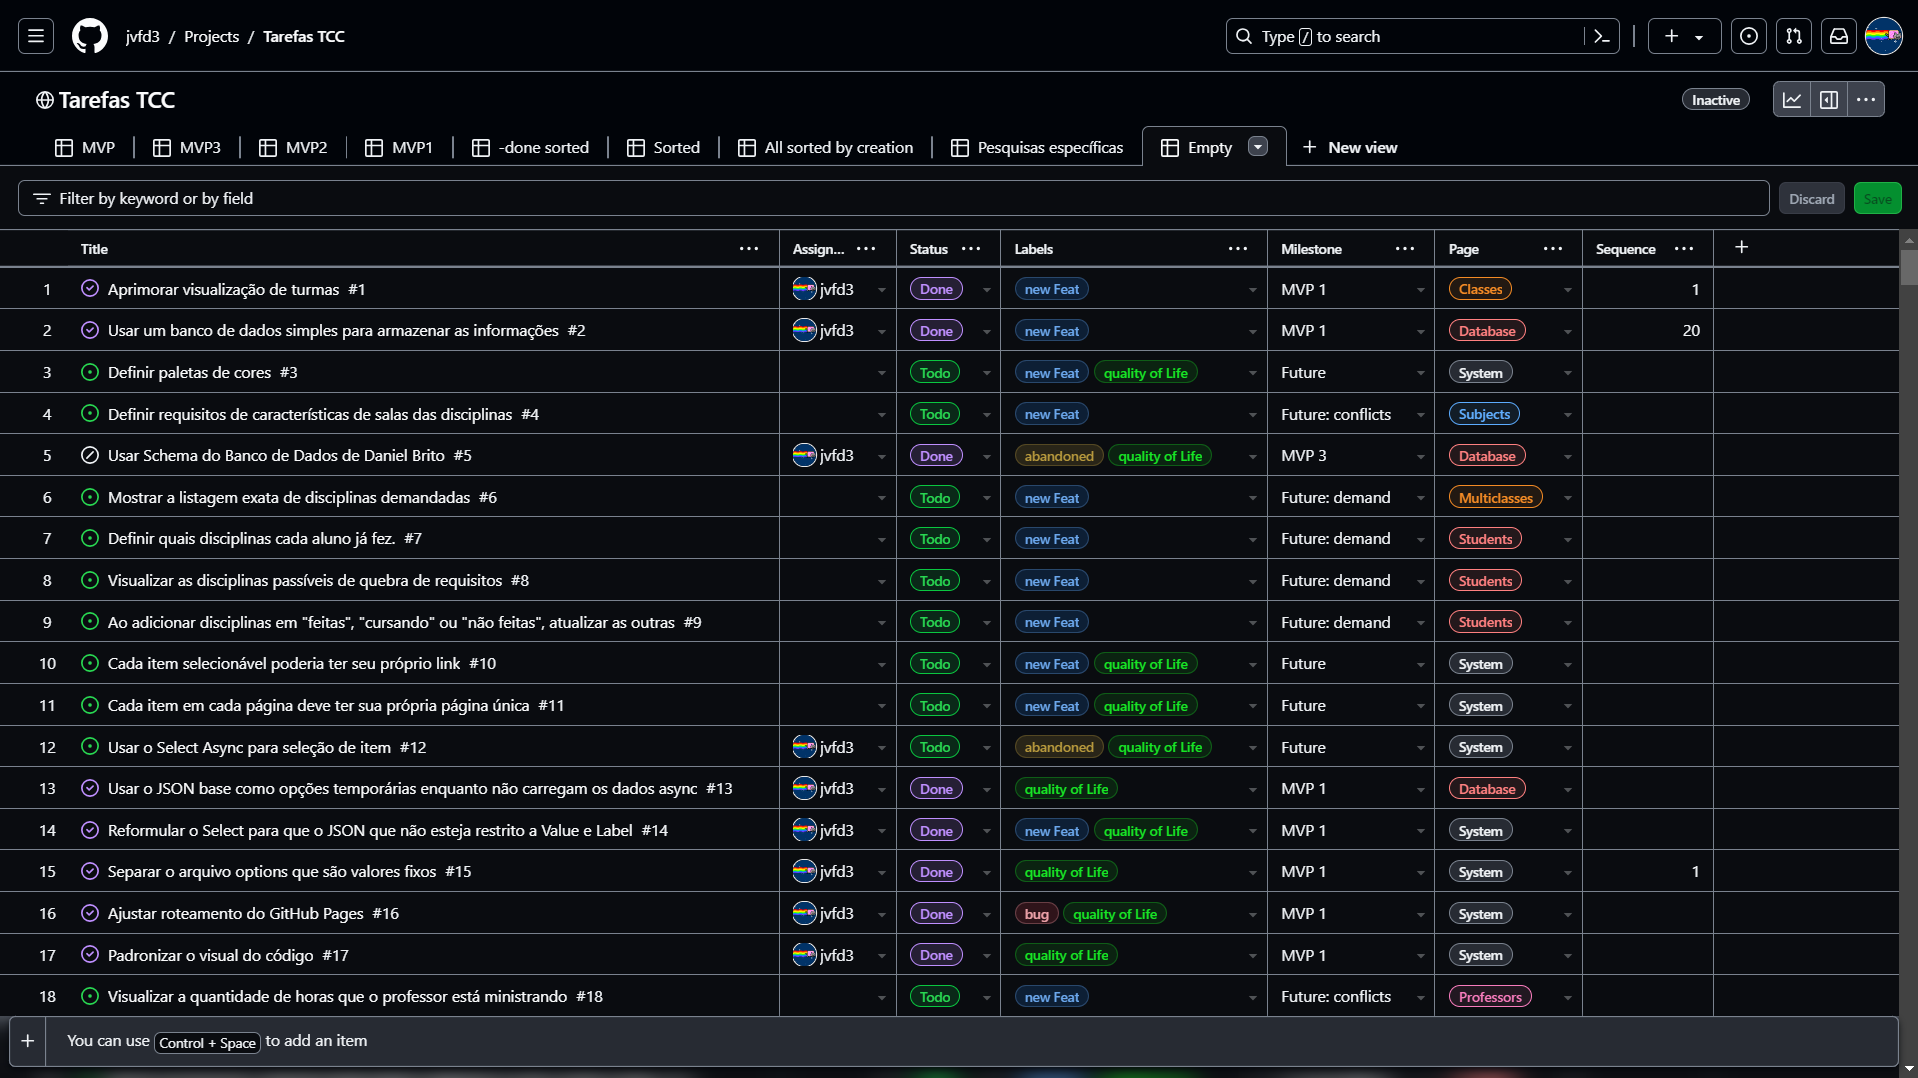
\includegraphics[width=\textwidth]{files/img/Codificacao/GitHubProjects - Table}
\end{MyCenteredFigure}

Tendo este novo sistema de tarefas em prática, foi possível tranquilizar a mente quanto ao conflito entre as funcionalidades que precisavam ser desenvolvidas, as que já estavam prontas, as que poderiam ter melhorias e quais se desejava implementar no futuro.

As tarefas foram inicialmente divididas em três principais categorias: \textit{Status}, \textit{Pages} e \textit{Sequence}. O \textit{Status} reflete o andamento da tarefa, se ela está disponível, em andamento, ou concluída. O \textit{Pages} reflete em qual página do sistema a tarefa se encontra, e o \textit{Sequence} reflete a ordem de prioridade da tarefa.

\subsubsection{Permanência dos Dados}

Tendo agora uma rota mais clara a ser seguida, o desenvolvimento foi retomado. Uma das características mais marcantes e ainda não atribuídas ao sistema era a manutenção dos dados. Para exemplificar o funcionamento geral da permanência dos dados, consideremos o uso de uma \textit{REST API} utilizando de 4 ``camadas'': o \textbf{\textit{frontend}}, os \textbf{\textit{endpoints}}, as \textbf{funções} de execução e o \textbf{banco de dados}.

O \textbf{\textit{frontend}} é a interface do sistema, onde o usuário interage com o sistema. Ele se encontra em duas formas: a primeira é o chamado ``em produção'', que é o sistema que o usuário final acessa, e a segunda é o chamado ``em desenvolvimento'', que é o sistema que o desenvolvedor acessa para realizar as modificações necessárias. Ambas precisam se comunicar com o \textit{backend} para realizar as quatro operações básicas no banco de dados (criação, leitura, atualização e deleção) por sobre as entidades existentes (turmas, professores, disciplinas, salas, etc.). Elas assim o fazer ao enviar requisições HTTP (\textit{GET}, \textit{POST}, \textit{PUT} e \textit{DELETE}), contendo pacotes de informações em formato JSON para os \textbf{\textit{endpoints}}.

Os \textbf{\textit{endpoints}} são as rotas que o \textit{backend} disponibiliza para a recepção das requisições HTTP. Eles são responsáveis por encaminhar as requisições recebidas. Se funcionamento é simples: rotear as requisições recebidas junto com sua carga útil. Para tanto, as rotas criadas refletem diretamente a qual entidade do banco de dados a requisição se refere, sendo então assim sabido qual \textbf{função} deve ser executada.

As \textbf{funções} são as responsáveis por executar as operações no banco de dados. Elas processam o pacote de informações recebido, e então realizam a operação desejada no \textbf{banco de dados}.

O \textbf{banco de dados} recebe a requisição, processa a operação, e então retorna o status da operação. Esse retorno é então repassado camada por camada, até chegar ao \textit{frontend}, onde o usuário final pode visualizar o resultado da operação.

\begin{MyCenteredFigure}
  \caption{Diagrama da progressão funcionamento da permanência dos dados}
  \label{fig:API}
  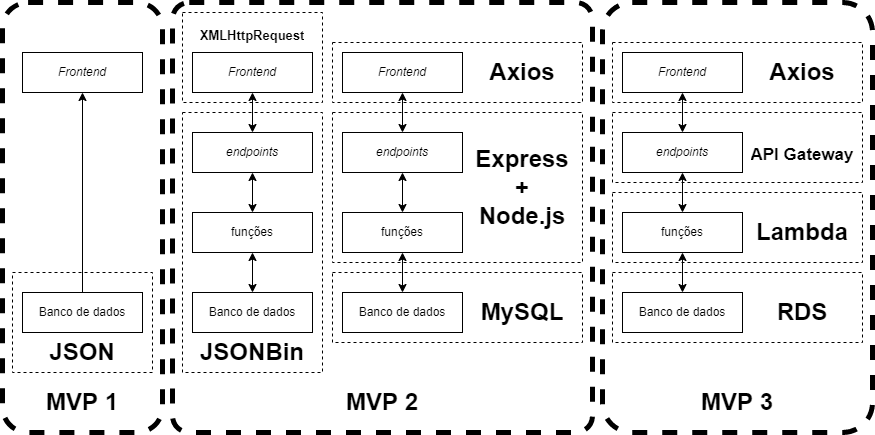
\includegraphics[width=\textwidth]{files/img/Codificacao/API - com diagrama}
\end{MyCenteredFigure}

\textbf{Resumidamente}: O \textbf{\textit{frontend}} envia uma requisição HTTP com uma carga de informações a um \textbf{\textit{endpoint}}, que encaminha a requisição a uma \textbf{função} específica que executa uma operação no \textbf{banco de dados}, assim retornando o status da operação ao \textit{frontend}. Essa sequência é ilustrada na \autoref{fig:API}.

\subsubsubsection*{\href{https://jsonbin.io/}{JSONBin}}

Como até então os dados estavam armazenados em formato JSON, imaginou-se que a melhor forma de persistir os dados seria através de um banco de dados que lidasse com JSON, e o escolhido foi o JSONBin.

Esta plataforma permite a criação de \textit{bins}, que são basicamente coleções de dados em formato JSON. A partir disso, é possível realizar requisições HTTP para a leitura, escrita, atualização e remoção dos dados. A utilização do JSONBin foi feita através de requisições HTTP usando o objeto \textit{XMLHttpRequest} do JavaScript, e a comunicação entre o \textit{frontend} e o JSONBin foi feita através de \textit{tokens} de acesso.

Com isso, se tornou possível ler e atualizar os dados de forma remota, e assim, manter os dados mesmo após a recarga da página. Embora cumprisse com o que promete e o que era desejado, o JSONBin não se mostrou a melhor escolha para o sistema, visto que a sua utilização não performou tão bem quanto se esperava. Não se sabe se foi por inexperiência ou por limitações do próprio serviço, mas a utilização do JSONBin para a coleta dos dados, fazia com que a tela de carregamento do sistema demorasse alguns segundos para ser exibida, o que não é apropriado para a usabilidade do sistema proposto.

\subsubsubsection*{MySQL}

Embora houvesse o desejo do uso de informações em formato JSON, achou-se por bem utilizar um banco de dados mais usual, recorrendo então ao MySQL, sendo então necessário criar um banco de dados local que armazenasse os dados e que pudesse ser acessado pelo sistema. Essa configuração serviu para estabelecer a supracitada camada de banco de dados. E consistiu basicamente na instalação do MySQL Server.

\paragraph*{Migração dos dados}

Como os dados se encontravam em formato JSON, primariamente utilizou-se da ferramenta de importação de dados do próprio \textbf{MySQL Workbench}. Durante essa importação, o software automaticamente identifica os campos, criando a tabela e suas colunas. Porém, devido à quantidade dos dados, essa importação tendia a ser demorada, e por vezes, falhava, sem haver uma explicação clara do porquê.

Com isso, foi necessário recorrer a uma abordagem semimanual, sendo então desenvolvido um código em Python que lê os arquivos JSON e os converte em arquivos SQL para que as \textit{queries} pudessem ser executadas no MySQL Workbench. A partir disso, foi possível importar os dados de forma mais rápida e eficiente.

Apesar da primeira tentativa de importação não ter sido completamente bem sucedida, foi desta forma que as tabelas, representadas pela \autoref{fig:TabelasIniciais}, foram inicialmente criadas. Não seguindo objetivamente a modelagem anteriormente citada. Isso gerou posteriormente a necessidade de ajustes manuais, como a adição de chaves primárias e estrangeiras, e a alteração de tipos de dados. Porém, como neste momento, o sistema visava apenas replicar o funcionamento do JSONBin, essas alterações não foram feitas de imediato.

\begin{MyCenteredFigure}
  \caption{Diagrama primitivo das tabelas de dados SQL}
  \label{fig:TabelasIniciais}
  
\includegraphics[scale=0.7]{files/img/Codificacao/DB inicial}
\end{MyCenteredFigure}

\paragraph*{Acesso ao Banco de Dados}

Seguindo a mesma sequência de camadas, o acesso ao banco de dados continua sendo feito através de requisições HTTP, porém, ao invés de serem enviadas ao JSONBin, são enviadas a um servidor local que executa as operações no banco de dados.

No \textit{frontend}, enquanto que para acessar a API já pronta do JSONBin foi utilizado o objeto \textit{XMLHttpRequest}, para a comunicação com o banco de dados local, foi utilizada a biblioteca \textit{Axios} para construir as requisições HTTP. E elas, ao invés de serem enviadas ao JSONBin, são enviadas ao \textbf{servidor local}.

Na criação deste \textbf{servidor local} utilizou-se a biblioteca \textit{Express} para desenvolver um \textit{backend} local executado paralelo ao \textit{frontend}. Essa biblioteca é responsável por criar todas as rotas necessárias para a comunicação entre o \textit{frontend} e o banco de dados. A partir disso, foi possível criar rotas para cada uma das entidades, e para cada uma das operações CRUD. Com isso, cada operação CRUD em cada uma das rodas é encaminhada para uma \textbf{função específica} que executa a operação no banco de dados.

Este uso, embora exemplifique a aplicação da permanência dos dados, está limitado por dois aspectos: em primeira instância, a permanência dos dados é limitada ao servidor local, não sendo este o desejo final do sistema. Em segunda instância, para haver o acesso aos dados, é necessário que, além do banco de dados, o \textit{backend} também esteja em execução, entretanto, o \textit{GitHub Pages}, onde o sistema está hospedado, não viabiliza essa execução. Com isso viu-se necessária a busca por um novo serviço de hospedagem.

\subsubsection{\textit{Amazon Web Services}}

Para suprir a necessidade de um servidor que pudesse executar o \textit{backend} do sistema em conjunto com o banco de dados, foi escolhido a \textit{Amazon Web Services} (AWS). A AWS é um serviço de computação em nuvem que oferece uma ampla gama de serviços, entretanto, apenas alguns deles foram necessários para o sistema.

O uso da AWS segue a mesma lógica do servidor local, com a diferença de que o servidor está em nuvem, e não localmente, assim resolvendo o primeiro dos dois problemas citados. Neste contexto o uso da AWS, representado pela \autoref{fig:APIAWS}, foi feito através de três serviços principais: o \textit{API Gateway} para a recepção das requisições HTTP, o \textit{Lambda} para a execução das funções que acessam o banco de dados, e o \textit{RDS} para o armazenamento dos dados; serviços estes que serão descritos mais detalhadamente a seguir.

\begin{MyCenteredFigure}
  \caption{API REST no AWS}
  \label{fig:APIAWS}
  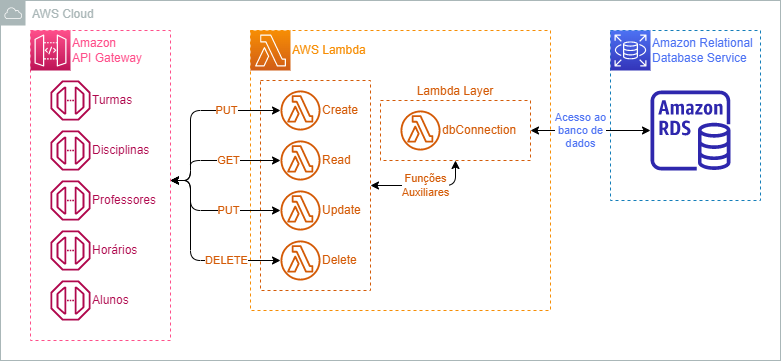
\includegraphics[width=\textwidth]{files/img/Codificacao/API-Funcionamento API.drawio}
\end{MyCenteredFigure}

O uso desses três serviços permitiu a execução do \textit{backend} do sistema em nuvem, e assim, atingindo a permanência dos dados. Com isso, o sistema passou a ser capaz de manter os dados mesmo após a recarga da página, e assim, atender a uma das principais necessidades do sistema.

% \subsubsubsection*{CORS} % Até agora não entendi direito pra que serve isso.

\subsubsubsection*{Implantação}

O conjunto de funcionalidades da AWS envolve em grande parte o objetivo de manter um sistema constantemente acessível através da internet, ainda assim, durante o desenvolvimento, ou até mesmo durante o ciclo de vida do software, é esperado que ocorram manutenções periódicas nas quais é compreensível que o sistema fique fora do ar. Sendo assim, para manter-se visando ao máximo a acessibilidade do sistema, espera-se que o mesmo fique desconectado o mínimo possível.

Tanto o API Gateway quanto as funções Lambda precisaram sofrer diversas modificações ao longo do desenvolvimento, e para que essas modificações fossem aplicadas. A aplicação dessas modificações é chamada de implantação (\textit{deploy}), onde a AWS substitui a versão atual do sistema pela nova versão. Essa aplicação de modificações foi inicialmente feita através da interface web da AWS, porém, com o tempo, foi percebido que essa abordagem era ineficiente. No caso do API Gateway, a ineficiência não era tão grande, visto que assim que as rotas estiverem configuradas, não há a necessidade de alterá-las. Já no caso das funções Lambda, cada mínima mudança no código requisitava um novo \textit{deploy} para cada uma das funções alteradas.

Outro detalhe percebido, foi que boa parte do código se repetia entre as funções que interagiam diretamente com o banco de dados. Sendo assim, passou-se a utilizar das \textit{Lambda Layers}, que são camadas que podem ser compartilhadas entre diversas funções, e assim, diminuir a quantidade de código repetido. Essa nova abordagem permitiu que as funções fossem mais enxutas, e que as mudanças fossem aplicadas de forma mais rápida, visto que bibliotecas e funções comuns entre as funções eram compartilhadas entre elas.

\subsubsubsection*{AWS CLI}

Nas primeiras tentativas de \textit{deploy}, duas abordagens eram utilizadas: a primeira era a de copiar e colar o código diretamente na interface web da AWS, e a segunda era a de fazer o upload de um arquivo zip contendo o código.

\begin{lstlisting}[caption={Código de \textit{deploy} de Lambda}, label={code:lambda}]
aws lambda create-function \
--function-name createProfessor \
--runtime nodejs20.x \
--role arn:aws:iam::375423677214:role/LambdaRole \
--handler index.handler \
--zip-file fileb://Files/AWS/lambdas/createProfessor/createProfessor.zip
\end{lstlisting}

Como mostrado no \autoref{code:lambda}, usa-se o software AWS CLI para criar uma função lambda. O comando \textit{create-function} é o comando que cria a função, e os argumentos que seguem são os parâmetros necessários para a criação da função. O \textit{function-name} é o nome da função, o \textit{runtime} é a versão do Node.js que a função utiliza, o \textit{role} é o conjunto de permissões criadas na seção \textit{AWS Identity and Access Management} (IAM), o \textit{handler} é o nome do arquivo principal que contém a função, e o \textit{zip-file} é o arquivo zip que contém o código da função.

Com isso, ao executar o comando, a função é criada, e então, a nova versão do código é aplicada. Com este fluxo de trabalho, embora permita o \textit{deploy} sem a direta conexão ao sistema AWS, ainda assim é necessário executar comandos específicos para cada uma, tendo que manualmente compactar o código e fazer o upload de cada um dos arquivos das diversas funções coexistentes.

\subsubsubsection*{SAM}

Como solução, foi utilizado o AWS SAM (\textit{Serverless Application Model}), que é uma extensão do \textit{AWS CloudFormation} que simplifica o desenvolvimento de aplicações sem servidor. O AWS SAM permite a definição de aplicações sem servidor de forma mais simples, e a partir disso, é possível fazer o \textit{deploy} de toda a aplicação de uma vez só. O uso do AWS SAM foi feito através de um arquivo \textit{template.yaml}, que contém a definição de todas as funções Lambda, e de recursos necessários para o funcionamento do sistema.

\lstinputlisting[language={YAML}, caption={\textit{Exemplo de template.yaml}}, label={code:template}]{files/codigos/AWS_SAM.yaml}

Como mostrado no \autoref{code:template}, o arquivo \textit{template.yaml} contém a definição de algumas das estruturas utilizadas para este sistema, principalmente as funções Lambda, visto que são quatro funções para cada uma das seis entidades, totalizando 24 funções. O arquivo contém a definição de cada uma das funções, e de cada uma das rotas que elas atendem. A partir disso, é possível fazer o \textit{deploy} de todas as funções que foram alteradas de uma vez só, e assim, diminuir o tempo de \textit{deploy} e a quantidade de comandos necessários.

Após o preparativo do arquivo \textit{template.yaml}, o \textit{deploy} é feito através do conjunto de comandos \textit{sam build; sam deploy}, que primeiro combina o \textit{CloudFormation Template} com o código da aplicação, e em seguida realiza o \textit{deploy} de todas as funções definidas no arquivo. Com isso, o sistema passou a ser mais facilmente atualizável, e mais facilmente mantido.

\subsubsection{Funcionalidades Adicionais}

Acrescendo à visualização de conflitos desenvolvida na primeira versão, foi implementada a visualização de conflito por capacidade de salas, ao comparar com a quantidade de alunos estimados para a turma. Mais detalhes sobre os conflitos podem ser vistos mais adiante na \autoref{sec:conflitos} denominada \nameref{sec:conflitos}.

Adicionou-se também diversas filtragens, principalmente na página de \textbf{Grade Horária}. Dessa forma, torna-se possível a visualização específica de turmas que atendam a certos critérios. Essa filtragem é feita através de caixas de seleção, onde é possível selecionar quais critérios se deseja filtrar, sendo eles: ano, semestre, categoria, disciplina, professor e sala. Essa coletânea de filtros viabiliza uma análise mais limpa das informações estruturadas, podendo então gerar \textit{insights} quanto ao posicionamento histórico das turmas.

Outra utilidade adicionada, agora na página \textbf{MultiTurmas}, foi a seção de ``Disciplinas ainda não oferecidas''. Sua funcionalidade consiste em dispor ao usuário uma lista de disciplinas que, segundo a ementa de Ciência da Computação, deveriam ser ofertadas naquele semestre. A partir disso, o usuário pode então selecionar o botão correspondente àquela disciplina e, a partir disso, uma turma para esta disciplina é adicionada à lista de turmas ofertadas. Há também um botão no topo que permite a adição de todas as disciplinas de uma vez.

\subsection{Terceira Versão} % ### 5.5.3. Terceira versão % https://github.com/jvfd3/timetabling-UENF/issues/348

Considerando que a segunda versão já apresentava em sua maioria as funcionalidades mínimas desejadas, a terceira versão foi focada em melhorias de usabilidade e na correção de bugs.

\subsubsection{Mudanças no \textit{GitHub Projects}}

O uso do GitHub Projects se provou como uma excelente forma de organização das tarefas, e assim, foi mantido para a terceira versão. Alguns novos detalhes foram adicionados em sua organização, como a adição da categorização de tarefas por \textbf{marcos} (\textit{milestones}, \autoref{fig:ProjectsMilestones}) e \textbf{etiquetas} (\textit{labels}, \autoref{fig:ProjectsLabels}).

\subsubsubsection*{Marcos e Etiquetas}

Os marcos visam distinguir as tarefas por suas versões, e também por seus tipos de funcionalidades futuras, assim, a medida em que surgiam novas ideias, elas eram adicionadas ao GitHub Projects. Então podemos considerar que cada um desses \textbf{marcos} teve tarefas atribuídas a si pois...

\begin{MyCenteredFigure}
  \caption{Marcos do GitHub Projects}
  \label{fig:ProjectsMilestones}
  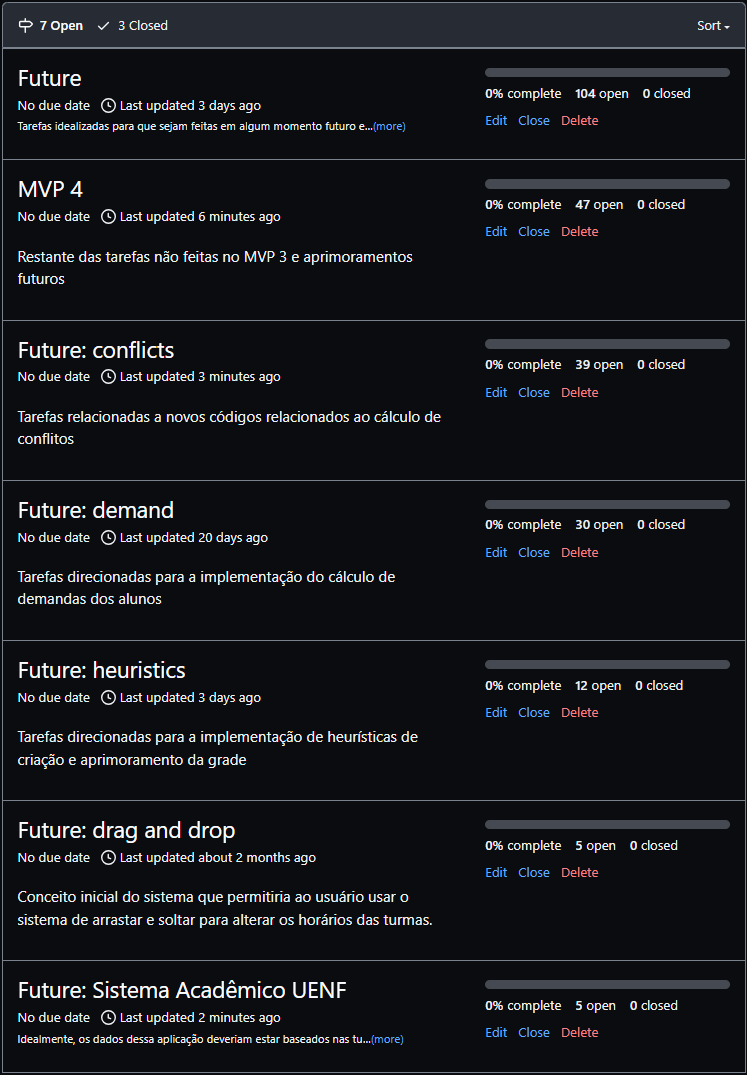
\includegraphics[scale=0.6]{files/img/Codificacao/GitHubProjects - Open Milestones}
\end{MyCenteredFigure}

\begin{enumerate}
  \item \textbf{MVP 1}: foram concluídas na primeira versão;
  \item \textbf{MVP 2}: foram concluídas na segunda versão;
  \item \textbf{MVP 3}: foram concluídas na terceira versão;
  \item \textbf{Futuro}: foram planejadas para o futuro do sistema;
        \begin{enumerate}
          \item \textbf{Demandas}: visam calcular a demanda dos alunos por disciplinas;
          \item \textbf{Conflitos}: visam aprimorar a visualização, qualidade e/ou variedade de conflitos;
          \item \textbf{Heurísticas}: visam aprimorar a alocação de turmas através de heurísticas;
          \item \textbf{Arrasta e solta}: visam aprimorar a alocação de turmas através de um sistema de arrastar e soltar;
          \item \textbf{Integração com o Sistema Acadêmico}: visam a integração do atual sistema com o sistema acadêmico da UENF.
        \end{enumerate}
\end{enumerate}

No Projects, também foram adicionadas as \textbf{etiquetas} que distinguem as tarefas por seu intuito.

\begin{MyCenteredFigure}
  \caption{Etiquetas do GitHub Projects}
  \label{fig:ProjectsLabels}
  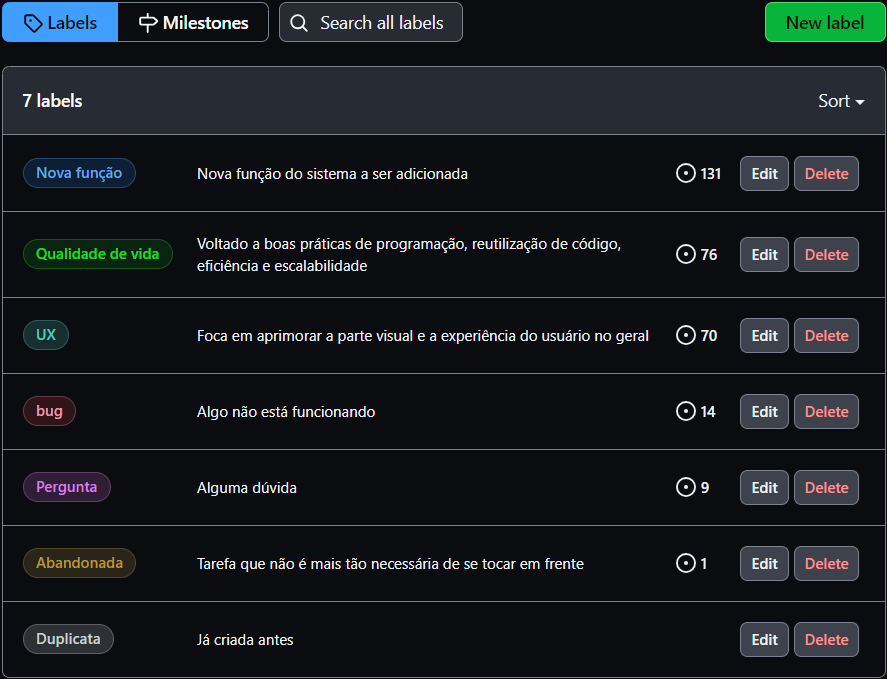
\includegraphics[scale=0.6]{files/img/Codificacao/GitHubProjects - Labels}
\end{MyCenteredFigure}

\begin{enumerate}
  \item \textbf{UX}: aprimoramento da experiência do usuário;
  \item \textbf{Bug}: correção de bugs;
  \item \textbf{Pergunta}: dúvidas sobre a validade da tarefa;
  \item \textbf{Duplicada}: já foi criada antes e que foi descartada;
  \item \textbf{Abandonada}: quando criada parecia interessante, mas que se decidiu por não implementar;
  \item \textbf{Qualidade de vida}: melhorias que não são necessárias, mas que aprimoram o processo de desenvolvimento;
  \item \textbf{Nova funcionalidade}: funcionalidades que ainda não foram implementadas;
\end{enumerate}

\subsubsubsection*{Gráficos}

O GitHub Projects também oferece a possibilidade de visualização de gráficos na seção \textit{Insights}, que mostram a quantidade de tarefas em cada uma das categorias. Esses gráficos são úteis para a visualização do andamento do projeto, e para a identificação de possíveis gargalos.

\begin{MyCenteredFigure}
  \caption{Gráfico de Marco \textit{versus} quantidade de tarefas separadas por etiqueta}
  \label{fig:ProjectsInsights}
  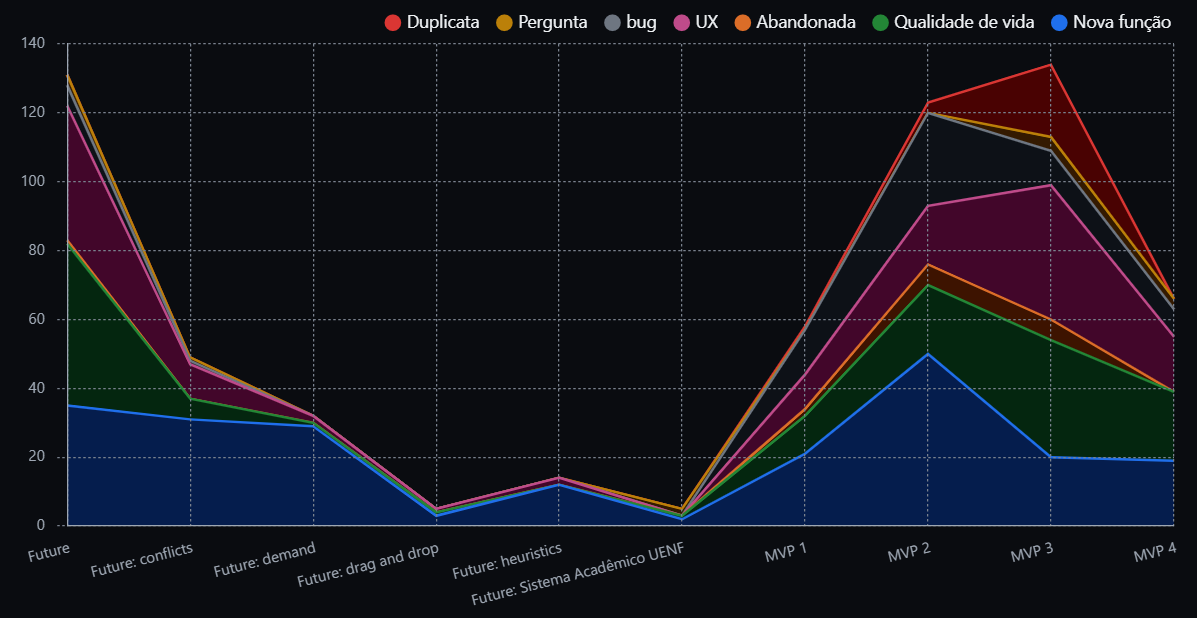
\includegraphics[width=\textwidth]{files/img/Codificacao/GitHubProjects - Insights - Stacked Line Milestone_Label}
\end{MyCenteredFigure}

Com eles, pode-se ter uma noção das métricas do projeto, como por exemplo:

\begin{itemize}
  \item Quantidade de tarefas de determinada etiqueta a cada marco, exemplificado na \autoref{fig:ProjectsInsights};
  \item Quantidade de tarefas por marco;
  \item Quais páginas receberam tarefas de quais etiquetas;
  \item Quantas são as tarefas em cada um de seus estados (Completas, em progresso, pendente).
\end{itemize}

\subsubsection{Melhorias no Sistema}

O sistema passou por diversas pequenas mudanças, e algumas maiores. Uma considerável parte delas foi relacionada à forma com que as informações eram estruturadas internamente, mudanças essas feitas com o intuito de tornar o sistema mais fácil de ser mantido posteriormente. Em seguida estão listadas algumas das várias melhorias feitas no sistema.

\subsubsubsection*{Filtros e ordenações}

Levando em consideração a multidimensionalidade da estrutura dos dados, a possibilidade de realizar ``curvas de nível'' e as ordenar por diferentes critérios se mostrou uma funcionalidade essencial para a compreensão dos dados. Dessa forma, em diferentes páginas do sistema, foram adicionadas ordenações padrões e seletores de filtragem manual, assim permitindo ao usuário a visualização de dados específicos.

Alguns exemplos de casos de uso dessas funcionalidades seria: ``Na página \textbf{MultiTurmas} o Professor A está tendo conflitos em suas turmas, então o usuário pode filtrar as turmas do Professor A e visualizar apenas as suas turmas. Em seguida, o usuário percebe que o Professor A está em conflito com a Sala B123, então o usuário visualiza apenas as turmas da Sala B123. Por fim, o usuário encontra um outro horário disponível para o Professor A e a Sala B123, e então, o conflito é resolvido.''

Uma das solicitações presentes ao final da versão anterior foi quanto a uma distinção mais clara entre disciplinas de Ciência da Computação e disciplinas de outros cursos. Para isso, embora não pareça apresentar grande robustez na forma como foi feito, apresenta suficiente clareza para o usuário final. A distinção foi feita ao utilizar o campo \textbf{Período Esperado} presente na entidade \textbf{Disciplina}, para definir que:

\begin{itemize}
  \item \textbf{1 $\leq$ Período Esperado $\leq$ 10}: Disciplina obrigatória de Ciência da Computação;
  \item \textbf{Período Esperado = 11}: Disciplina eletiva optativa para Ciência da Computação;
  \item \textbf{Período Esperado = 12}: Disciplina eletiva livre para Ciência da Computação;
  \item \textbf{Período Esperado = 13}: Disciplina não ofertada para Ciência da Computação;
\end{itemize}

Com essa divisão, definiu-se o sistema para que, por padrão, apenas exibisse as turmas voltadas para Ciência da Computação, e que, caso o usuário desejasse, poderia visualizar as turmas de outros cursos.

\subsubsubsection*{MultiTurmas}

Dentre as tarefas realizadas, uma das páginas que mais sofreu alterações foi a página de \textbf{MultiTurmas}. Nela, foram feitas diversas melhorias, como a adição de filtros, ordenações e aprimoramento dos textos contidos nas caixas de seleção.

\paragraph*{Aprimoramento dos identificadores dos conflitos}

Os conflitos ocorridos indicavam quais eram os identificadores (ids) das turmas que estavam em conflito, porém, esses ids eram os ids referentes ao banco de dados, sendo ele um valor numérico, não continha valor semântico suficiente para ser facilmente identificado. Estes ids eram visualizados ao posicionar o ponteiro do mouse por sobre os componentes cujo conflito foi verificado. Com isso, foi feita a adição de um novo identificador, que é composto pelas informações contidas na turma, sendo elas o ano, semestre, nome da disciplina, nome do professor, e o código descritor da turma. A partir disso, tornou-se mais fácil identificar quais turmas estavam em conflito, e assim, corrigi-las. Essa identificação foi adicionada também aos horários, onde o identificador passou a ser composto pela sala, dia da semana, horário de início e fim.

\paragraph*{Criação e deleção de turmas e horários}

Embora seja uma funcionalidade básica e existente desde a primeira versão, a criação e deleção de turmas apresentou diversos problemas ao longo do desenvolvimento. Um dos mais cruciais era devido à assincronicidade intrínseca ao uso de um banco de dados remoto. O problema era que durante a criação sequencial de duas turmas, apenas a segunda era mostrada, mesmo que ambas tivessem sido criadas.

O que ocorria era que, ao começar com a lista de $Turmas = [A, B]$ tenta-se adicionar a turma $C$ à lista de $Turmas$, mas para isso, a requisição enviada ao banco de dados deve retornar com o status de sucesso, e para que, só assim, fosse adicionada à listagem apresentada no sistema. Então, caso fosse feita a tentativa de se adicionar a turma $D$ antes da confirmação anterior ser recebida, a adição seria realizada novamente na listagem inicial ($[A, B]$). Por fim, assim que a primeira requisição retornasse bem sucedida, por um breve instante a listagem seria $[A, B, C]$, e então, após a adição da turma $D$, a listagem seria $[A, B, D]$.

Para resolver esse problema, foi feita a adição de uma função de \textit{callback} que passou a utilizar o estado mais atual da listagem de turmas, e não mais a listagem inicial.

Outra característica aprimorada, foi a velocidade de adição e deleção, principalmente a de deleção. Antes, a aprovação do banco de dados era necessária para que a lista de turmas fosse atualizada, e isso tornava o processo de deleção lento. Para resolver isso, foi feita a adição de uma função de deleção que remove a turma da listagem de turmas antes mesmo da confirmação do banco de dados. Essa não se mostra como a solução mais adequada, visto que em caso de falha na deleção, a turma poderá ser restaurada com a simples atualização da página, os pontos positivos na usabilidade superam os negativos.

\paragraph*{Adição da propriedade \textbf{descrição}}

Disciplinas oferecidas em um mesmo semestre por vezes são oferecidas para alunos demais para que uma única turma os comporte, e assim, é necessário a criação de mais de uma turma. Para que os alunos e professores possam identificar facilmente a qual turma pertencem, foi adicionada a propriedade descrição, que é uma breve descrição da turma. Essa característica já se encontra no sistema acadêmico, porém com a limitação de apenas 3 caracteres. No presente trabalho, a descrição pode conter até 255 caracteres.

Adicionando esse campo, a visualização linear das informações da turma se tornou mais difícil de se manter na tela. Considerando que em sua maioria as turmas possuem dois horários, dispôs-se então as informações em conjuntos de dois elementos, ao invés de uma lista única, tornando então a visualização mais densa.

\paragraph*{Solução inicial}

A funcionalidade anteriormente denominada ``Disciplinas ainda não oferecidas'' foi aprimorada de tal forma que agora, além de criar uma turma para a disciplina selecionada, o sistema automaticamente analisa o histórico de criação de turmas, definindo previamente o professor, a demanda estimada, e os horários, incluindo seus dias, horas de início e sala em que é alocada.

O cálculo da demanda estimada é dado pela média de demandas de todas as turmas anteriores que possuem demanda estimada. Entretanto, atualmente apresenta-se desativada.

% Lembrar de reativar essa funcionalidade.

O botão de adição de todas as disciplinas foi mantido, e agora, ao ser clicado, cria as turmas com suas características já preenchidas, não considerando, entretanto, a descrição, visto que esta é uma característica única de cada turma e deve ser adicionada manualmente em caso de necessidade. Então, após a criação de todas as turmas referentes ao curso de Ciência da Computação, uma solução inicial foi obtida.

É esperado, entretanto, que esta solução apresente problemas em sua execução, visto que nem todas as alocações de turmas apresentam um padrão. Então, fica a cargo do usuário a verificação e a correção dos possíveis erros alertados pelo sistema.

\subsubsubsection*{Grade Horária}

A página que detinha o nome ``CCTable'' e que visava apresentar exclusivamente as disciplinas do curso de Ciência da Computação, foi renomeada para ``Grade Horária'', e passou a ser possível de apresentar disciplinas de todos os cursos, embora ainda não seja possível distinguir as disciplinas de um curso para o outro.

As células das turmas sofreram um ligeiro aprimoramento visual e foram ordenadas primariamente por seu período esperado.

\subsubsubsection*{Banco de dados}

Quanto ao banco de dados, os dados antes desconexos passaram a ser interligados adequadamente por chaves estrangeiras. Apresentando então restrições em casos de deleções inapropriadas no banco de dados. A API, por sua vez, deixou de retornar as listas de turmas, professores, disciplinas e salas, e passou a retornar os dados de forma mais estruturada em formato JSON.

\paragraph*{Preenchimento de dados}

Inicialmente, os dados adicionados faziam jus diretamente às disciplinas, professores, salas e turmas do curso de Ciência da Computação. Porém, como para a análise completa dos conflitos é necessário que seja feita também a adição das turmas de outros cursos, foi feito o preenchimento de dados para as entidades de professores, disciplinas e salas.

Para acumular mais dados referentes às entidades do banco de dados, foram tomadas algumas abordagens: requisição dos dados diretamente do Sistema Acadêmico, processamento de tabelas, processamento de PDFs e \textit{web scraping}, todos eles ilustrados pela \autoref{fig:DataFlow}.

\begin{MyCenteredFigure}
  \caption{Diagrama do fluxo de obtenção de dados}
  \label{fig:DataFlow}
  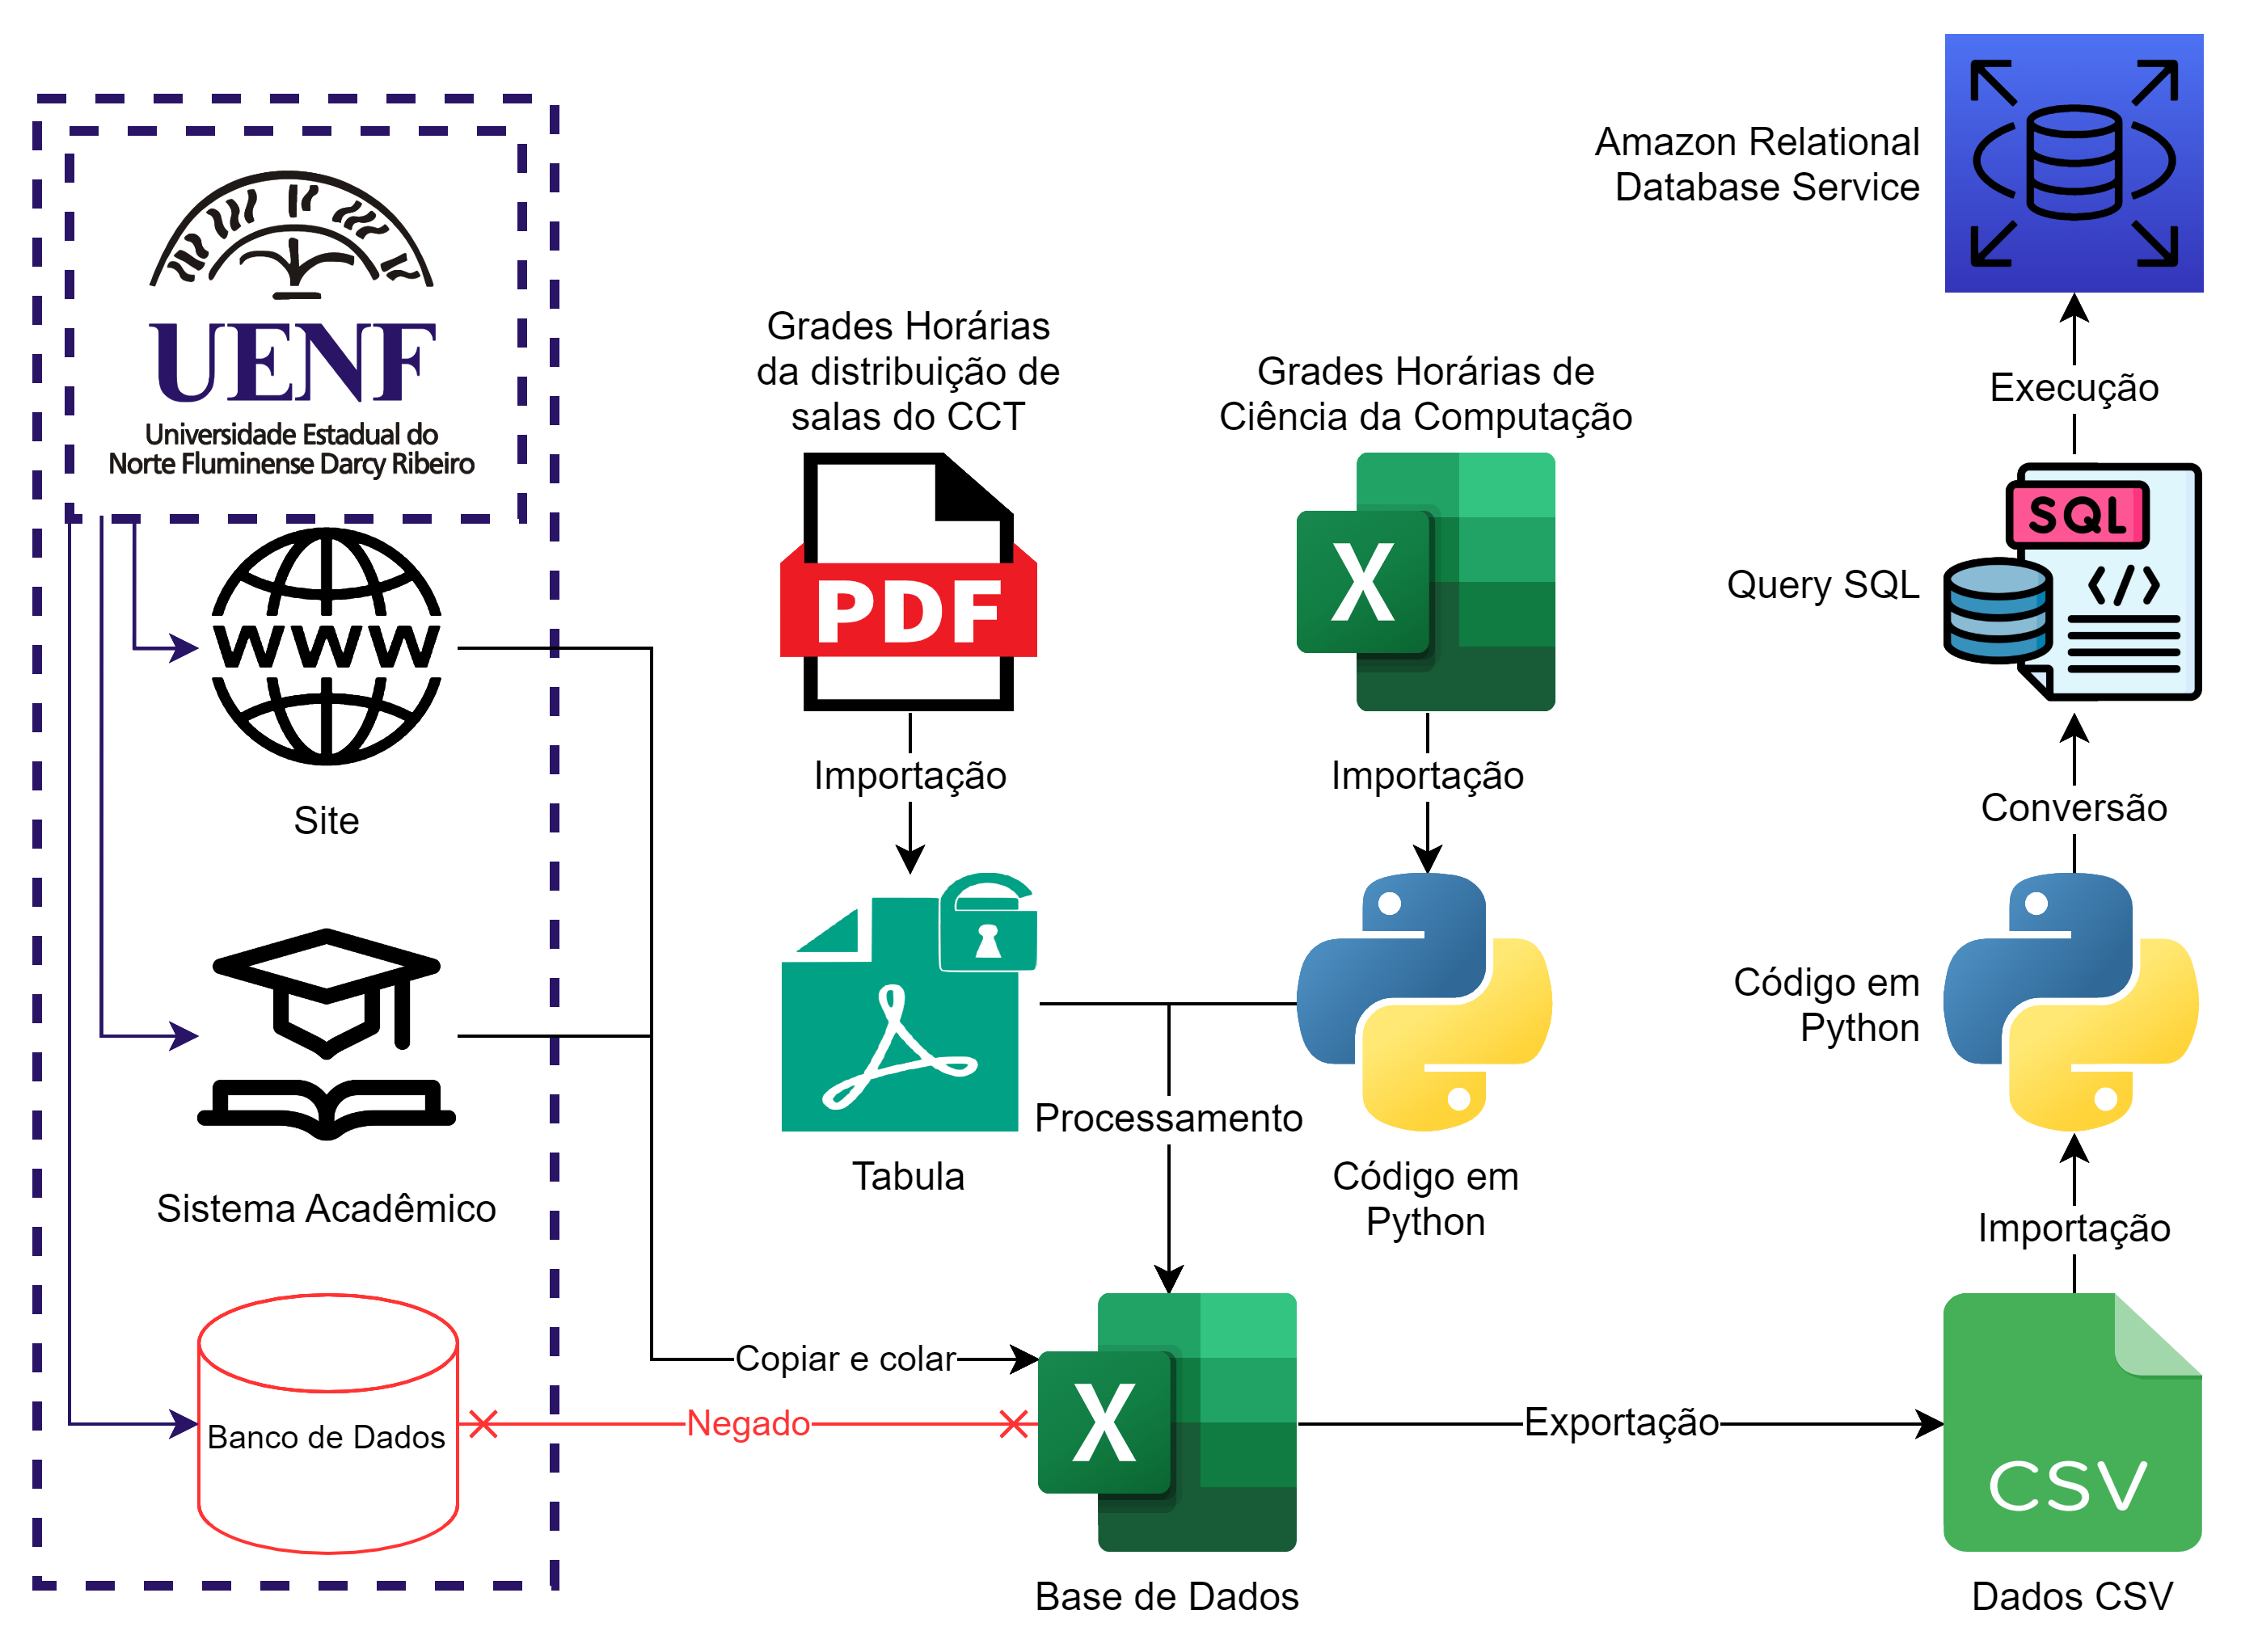
\includegraphics[width=\textwidth]{files/img/Codificacao/Processamento de dados.drawio}
\end{MyCenteredFigure}

A forma teoricamente mais direta e eficiente para se obter os dados das entidades é a obtenção das informações contidas no banco de dados do sistema acadêmico. Para este fim, foi feita uma solicitação ao responsável pela Secretaria Acadêmica (SECACAD) da UENF, que direcionou a solicitação ao desenvolvedor do Sistema Acadêmico. A resposta obtida do desenvolvedor foi que a solicitação não poderia ser atendida, visto que não detinha a posse dos dados, e que para que pudesse fornecê-los, seria necessária uma solicitação formal à reitoria da UENF. Essa solicitação foi então passada à Coordenação do curso de Ciência da Computação, com o qual ficou decidido abandonar a ideia e buscar outras formas de obtenção dos dados.

Paralelamente à abordagem anterior foram feitas tentativas individuais de obtenção dos dados. O processamento de tabelas e PDFs e o \textit{web scraping} foram as abordagens utilizadas. Inicialmente os dados foram coletados e armazenados em tabelas, e então, convertidos para o formato CSV. Os arquivos CSV, por sua vez, foram utilizados em \textit{scripts} Python que os convertiam em \textit{queries} SQL, para que assim então fossem adicionados ao banco de dados.

Os PDFs analisados dispunham de tabelas referentes à oferta de turmas para o CCT, mas os dados advindos do processamento de PDF não são tão estruturados quanto os de uma tabela Excel, por este motivo, a primeira abordagem foi a solicitação dos arquivos tabulares para aquele que os produziu. Não havendo resposta favorável quanto a isso, diversos \textit{softwares} de conversão de tabelas em PDF para Excel foram testados, porém, nenhum deles foi capaz de converter as tabelas de forma satisfatória. Um dos agravantes é a existência de células mescladas, o que torna mais complicada a conversão direta. Outra abordagem testada foi a de importação direta dos PDFs através do Excel e também o simples copiar e colar. Nenhum desses métodos foi eficiente, então com isso alguns dados foram coletados, mas sem certeza quanto à sua precisão. Deste método foram coletadas as informações referentes à nomes de professores e disciplinas, capacidades das salas, e horários de aulas.

Além dos PDFs anteriores, haviam também os arquivos referentes à oferta de turmas para o curso de Ciência da Computação. Estes sim dispunham também de sua versão em Excel, e assim, foram processados utilizando \textit{scripts} Python. A abordagem apresentou falhas, visto que a notação das informações não apresentava o mesmo padrão ao longo dos anos, então foi necessário fazer ajustes manuais, resultando em uma tabela normalizada com diversas pastas de trabalhos referentes a cada um dos semestres desde 2019, não considerando os semestres de verão. Deste método foram coletadas as informações referentes à nomes e apelidos de professores e disciplinas, demandas estimadas dos alunos pela turma, descrição da turma, e horários de aulas.

Por fim, foi feita o \textit{web scraping} que consistiu na busca por informações em diversos sites, principalmente o \href{https://academico.uenf.br/usuarios/sign_in}{Sistema Acadêmico}, o \href{https://uenf.br/portal/}{site da UENF} e outros sites. Nessa etapa, foi possível encontrar lotes de informações estruturadas. Um dos lotes foi a listagem de disciplinas e suas características que se encontram disponíveis no Sistema Acadêmico da UENF, essas informações foram copiadas e coladas no arquivo Excel unificado. Outros lotes foram encontrados dispersos ao longo do site da UENF e consistiam basicamente em listagem de professores e seus respectivos laboratórios. Essas informações estavam dispersas dos sites dos diversos centros e cursos, alguns disponíveis no próprio site, outros em formato de arquivo. Deste método foram coletadas as informações referentes à nomes de professores, seus laboratórios e centros; e disciplinas e seus nomes, códigos e períodos de vigência. Além disso, foram encontrados documentos oficiais que referenciam a capacidade de ocupantes das ``salas'' disponíveis do Centro de Convenções, popularmente conhecido como ``Apitão'' que mesmo não sendo propriamente uma sala de aula, já foi utilizado previamente para tal fim. Outras salas já obtiveram alocações similares, assim como a Sala dos Professores.

\subsubsubsection*{Gerais}

Neste tópico estão descritas algumas melhorias gerais do sistema que não se enquadraram nos tópicos anteriores.

\paragraph*{Aprimoramento na forma de criação de itens}

Antes, ao acessar a página de criação de entidades, uma entidade era previamente selecionada. E para a criação de uma nova entidade, os valores da entidade anterior deveriam ser alterados, e, ao clicar em adicionar, esses valores alterados eram cadastrados no banco de dados. Essa sequência de ações apresentou intuitividade suficiente e, portanto, foi alterada.

A versão atual passou a não selecionar previamente a entidade. Assim, ao clicar em adicionar um novo item, uma nova entidade é criada. No caso das turmas, a entidade é criada com os valores de ano e semestre predefinidos baseado na filtragem selecionada.

\paragraph*{Boas práticas}

Além das funcionalidades voltadas para o usuário final, algumas mudanças classificadas como \textbf{Qualidade de vida} foram realizadas visando a manutenção do sistema. Dentre elas estão:

\begin{itemize}
  \item \textbf{Repadronização de componentes}: como o conhecimento relacionado a boas práticas de programação foi adquirido ao longo do desenvolvimento, partes de componentes criados anteriormente foram reformulados para que estivessem estruturados de acordo com a estrutura recentemente desenvolvida no código.
  \item \textbf{Externalização de informações}: algumas informações constantes como cores de fundo e textos foram externalizadas para variáveis, assim, caso haja a necessidade de alteração, não será necessário a busca manual por todas as ocorrências. Um outro caso desses é referente aos textos dispostos nas caixas de seleção, que foram convertidos em funções que retornam o texto desejado.
  \item \textbf{Inglês}: como as linguagens de programação de modo geral se apresentam no idioma inglês, é considerado uma boa prática que as variáveis e funções também, o que não foi a abordagem inicialmente tomada. Assim, foi feita uma gradual migração para o inglês, e embora não tenha sido concluída, a maior parte do código já se encontra em inglês. Para facilitar essa migração, foi elaborado um sistema de ``\textit{getters}'' como forma de obter a propriedade de determinado objeto, independente de qual língua ele esteja.
  \item \textbf{Remoção de estruturas obsoletas}: ao longo do desenvolvimento, algumas estruturas foram criadas e não utilizadas. Um exemplo dessas foi a propriedade ``Ordem'' que visava definir a ordem em que os horários da turma apareceriam, porém o resultado desta propriedade foi obtido com a ordenação dos horários por dia e em seguida por horário, não sendo então necessária. Ela então foi removida do sistema e do banco de dados.
\end{itemize}

\section{Conflitos}\label{sec:conflitos} % ### 5.6. Conflitos

Uma das principais funcionalidades do sistema é a detecção de conflitos. Seu objetivo é auxiliar ao usuário a identificar possíveis problemas na alocação das turmas, e assim, permitir que ele possa corrigi-los antes de finalizar a grade horária. Diversas situações podem ser consideradas como conflitos, e cada uma delas é tratada de forma diferente.

Os conflitos aqui se colocam como uma forma de alerta ao usuário, e não como uma restrição, assim viabilizando ao usuário que uma ação seja tomada, ou não, a partir do alerta. O conceito da não restrição é importante, visto que embora idealmente espera-se que o processo de alocação disponha de todas as informações para que seja otimamente alocado, na prática, isso atualmente não se mostra uma realidade.

Essa flexibilização das restrições que poderiam ser tidas como rígidas em um problema de otimização, é uma característica do problema de alocação de turmas da UENF. A flexibilidade é necessária, visto que o processo de alocação é feito de forma manual. Além disso, diversos casos atípicos acabam por ocorrer na realidade da universidade, e que, embora possam não ser aconselháveis ou até mesmo tidos como conflituosos pelo sistema, não seriam de fato um problema para a execução prática das alocações.

\subsection{Típicos Conflitos Atípicos}

Para ilustração, abaixo estão descritos alguns exemplos de conflitos que poderiam ser alertadas pelo sistema, mas que não seriam realmente um restritor para a execução prática das alocações:

Considerando o diminuto corpo docente do curso de Ciência da Computação, que atualmente conta com seis professores doutores, é recorrente a solicitação de professores bolsistas para ministrar disciplinas. Devido aos prazos existentes ao longo do processo de criação da grade horária, é comum que ainda não se saibam quais e quantos professores bolsistas serão disponibilizados para quais turmas. Porém, como o Sistema Acadêmico requere a inserção de professores para a criação de turmas, uma solução encontrada foi a inserção de um desses professores permanentes como responsável pela turma. E, mesmo após se obter a informação quanto a quais e quantos bolsistas estarão disponíveis, ainda assim o sistema acadêmico não os permite serem inseridos, visto que eles não têm um vínculo permanente com a instituição. Com isso, seria possível ver, por exemplo, um conflito entre duas turmas que possuem o mesmo professor em um mesmo horário, mas que na prática, uma delas será ministrada por um professor bolsista.

Outras situações que podem ocorrer revolvem em torno da alocação das salas. Duas situações que podem ilustrar sua atipicidade são: a possibilidade de alocar uma turma a uma determinada sala, mesmo que se tenha a intenção de ministrá-la em outra, e também a possibilidade de se repartir a turma em duas salas de aula ocorrendo simultaneamente.

Esses e outros são exemplos de situações recorrentes ao longo do processo flexível da organização da tabela horária.

\subsection{Conflitos Tratados pelo Sistema}

Para a implementação, primeiro visou-se a detecção de conflitos que poderiam ser considerados restritores para a alocação das turmas. Sendo eles os de alocação simultânea de salas e professores, visto que um professor não pode ministrar duas turmas simultaneamente, nem uma sala deve comportar duas turmas simultaneamente (embora ambos sejam teoricamente possíveis).

Além disso, também foi implementada a detecção de conflitos de capacidade, onde a quantidade de alunos de uma turma é maior do que a capacidade da sala alocada, e alguns outros indicativos visuais que serão descritos abaixo.

Os conflitos calculados são representados de três formas diferentes. A primeira e mais perceptível é a mudança de cor de fundo das propriedades conflituosas. A segunda, visando evitar sobreposição de conflitos, é a adição de uma borda inferior que se estende por toda a largura da propriedade. E a terceira, mais descritiva, é o uso do atributo \textit{title} dos elementos HTML, que exibe uma mensagem de alerta flutuante ao passar o mouse sobre a propriedade conflituosa, assim dispondo de mais detalhes sobre os conflitos buscados e encontrados. % "propriedades conflituosas" é um bom termo?

Embora o sistema seja projetado para ser permissivo quanto a inexistência de certas informações, é sempre esperado que a maior quantidade de informações possíveis seja inserida, assim, caso algum campo não tenha sido preenchido a cor de fundo do elemento será alterada para um tom acinzentado.

\begin{MyCenteredFigure}
  \caption{Paleta de cores do sistema}
  \label{fig:conflitoDisciplinaPaleta}
  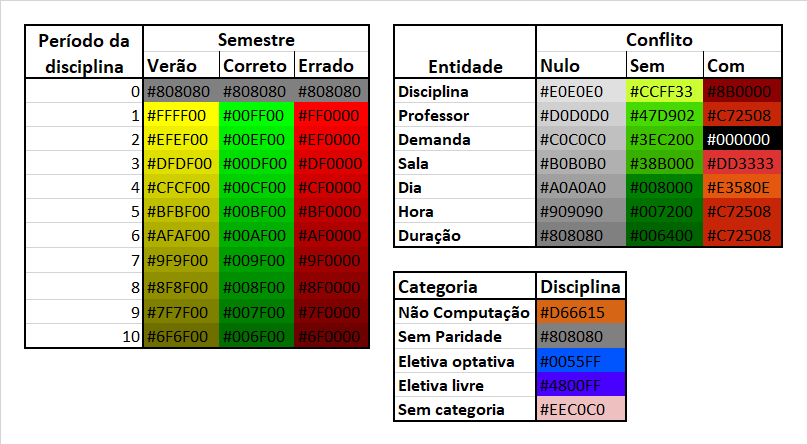
\includegraphics[width=\textwidth]{files/img/Codificacao/Conflitos/Paleta de Cores}
\end{MyCenteredFigure}

Os conflitos que são representados por cores, têm sua paleta de cores representada na \autoref{fig:conflitoDisciplinaPaleta}. Nessa paleta, dispõe-se de 3 conjuntos principais: a distribuição de cores para as disciplinas obrigatórias do curso de Ciência da Computação, que variam de acordo com o semestre em que são ofertadas; a categoria das disciplinas não obrigatórias para o curso de Ciência da Computação; e os conflitos das outras entidades, que são classificados amplamente entre ``com conflito'', ``sem conflito'' e ``conflito nulo''.

\subsubsection{Professores}

O sistema contempla a checagem de conflitos de alocação simultânea de professores em mais de uma turma. Ou seja, considerando todas as turmas ao qual o professor está atribuído no ano e semestre selecionados, o sistema compara todos os horários das turmas deste professor, e verifica se há alguma interseção entre horários que estão no mesmo dia, levando em conta a duração da aula.

\begin{MyCenteredFigure}
  \caption{Exemplo de conflito de alocação de professor}
  \label{fig:conflitoAlocacaoProfessor}
  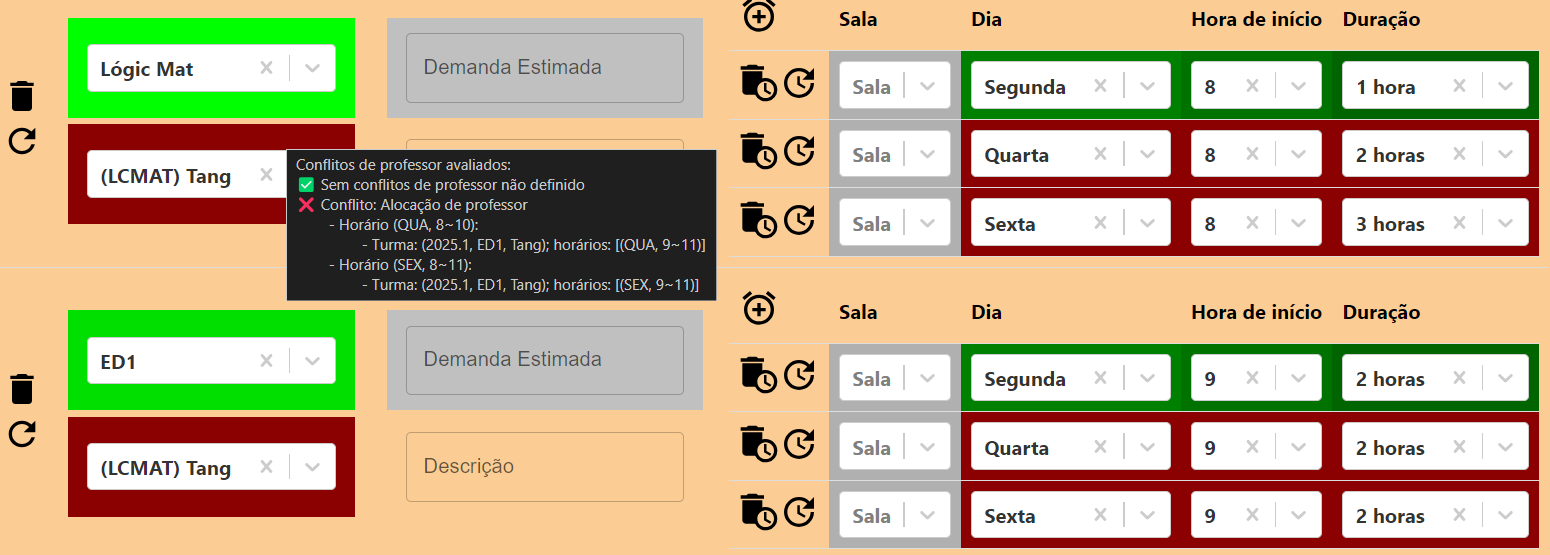
\includegraphics[width=\textwidth]{files/img/Codificacao/Conflitos/Alocação de professores}
\end{MyCenteredFigure}

Caso haja algum conflito, o sistema destaca o professor em questão, tornando a sua cor de fundo avermelhada. Além disso, ao passar o mouse sobre o nome do professor, é exibido um alerta flutuante, informando que quais são as turmas e horários que estão em conflito. Esse comportamento é exemplificado na \autoref{fig:conflitoAlocacaoProfessor}, onde o professor Tang é alocado em duas turmas que ocorrem simultaneamente durante algum intervalo de tempo durante os horários de quarta e sexta-feira, assim informando no alerta flutuante quais são as turmas e horários que estão alocados simultaneamente.

\subsubsection{Salas}

As salas também apresentam a verificação do conflito de alocação simultânea. Porém, diferente dos professores, a checagem é feita conferindo todos os horários na qual a sala está alocada, e então é feita a mesma verificação de interseção citada anteriormente. Havendo o conflito, é exibida uma borda alaranjada na parte inferior das propriedades referentes ao conflito, além de, assim como no caso dos professores, exibir o alerta flutuante. A \autoref{fig:conflitoAlocacaoSalas} representa um caso de conflito de alocação de salas.

\begin{MyCenteredFigure}
  \caption{Exemplo de conflito de alocação de sala}
  \label{fig:conflitoAlocacaoSalas}
  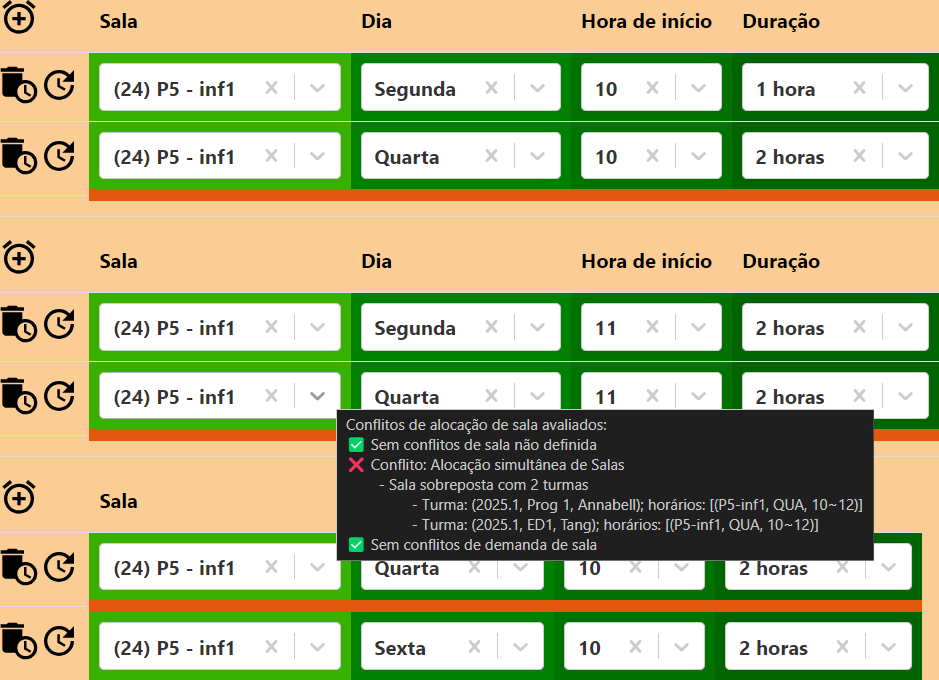
\includegraphics[width=\textwidth]{files/img/Codificacao/Conflitos/Alocação de Salas - Sala}
\end{MyCenteredFigure}

Além disso, também é feita a comparação entre a quantidade máxima de alunos comportados na sala e a quantidade de alunos estimados para a turma. Este conflito por sua vez é ilustrado tornando avermelhado o fundo da demanda estimada e da seleção de salas. Caso uma turma tenha mais de um horário, é calculada a quantidade remanescente dos alunos que demandam a disciplina com relação a cada uma das capacidades das salas destes horários, mostrando cada um deles no alerta flutuante.

Então, como pode-se perceber na \autoref{fig:conflitoAlocacaoSalasCapacidade}, a turma fictícia que apresenta demanda estimada de 31 alunos não poderia ser adequadamente alocada às salas ``P5 - inf1'', nem na ``P3 - Bcct'', visto que a primeira apenas comporta 24 alunos e a segunda, 30 alunos. O alerta flutuante, ao ser acionado, informa ainda quantos são os alunos que não poderiam ser alocados em cada uma das salas.

\begin{MyCenteredFigure}
  \caption{Exemplo de conflito de capacidade na sala}
  \label{fig:conflitoAlocacaoSalasCapacidade}
  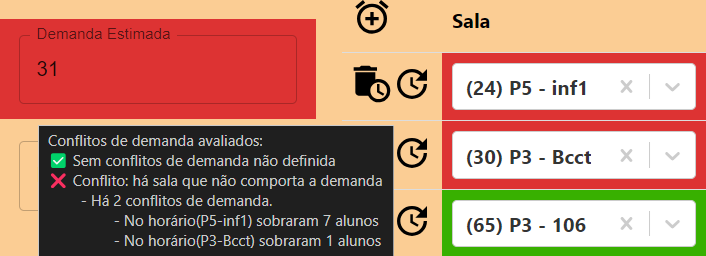
\includegraphics[width=\textwidth]{files/img/Codificacao/Conflitos/Demanda X Capacidade}
\end{MyCenteredFigure}

\subsubsection{Disciplina}

Além desses conflitos, outras características analisadas e representadas se referem às disciplinas atribuídas às turmas, que, embora não representem necessariamente um \textit{conflito}, mas sim um indicativo, ainda assim serão tratados como conflitos por motivos de simplificação. Esse indicativo leva em consideração o semestre selecionado e o período esperado da disciplina de certa turma. Utilizando de lógica similar, também é indicado caso não tenha sido atribuído um período à disciplina, e se, para o curso de Ciência da Computação, a disciplina é considerada como \textbf{Eletiva Livre}, \textbf{Eletiva Optativa}, ambas em tons azulados, ou se não é uma disciplina para o curso de Ciência da Computação, sendo então representada em tons alaranjados. Estas características são ilustradas no lado direito da \autoref{fig:conflitoDisciplinaTitulos}.

\begin{MyCenteredFigure}
  \caption{Avisos flutuantes dos conflitos de disciplinas}
  \label{fig:conflitoDisciplinaTitulos}
  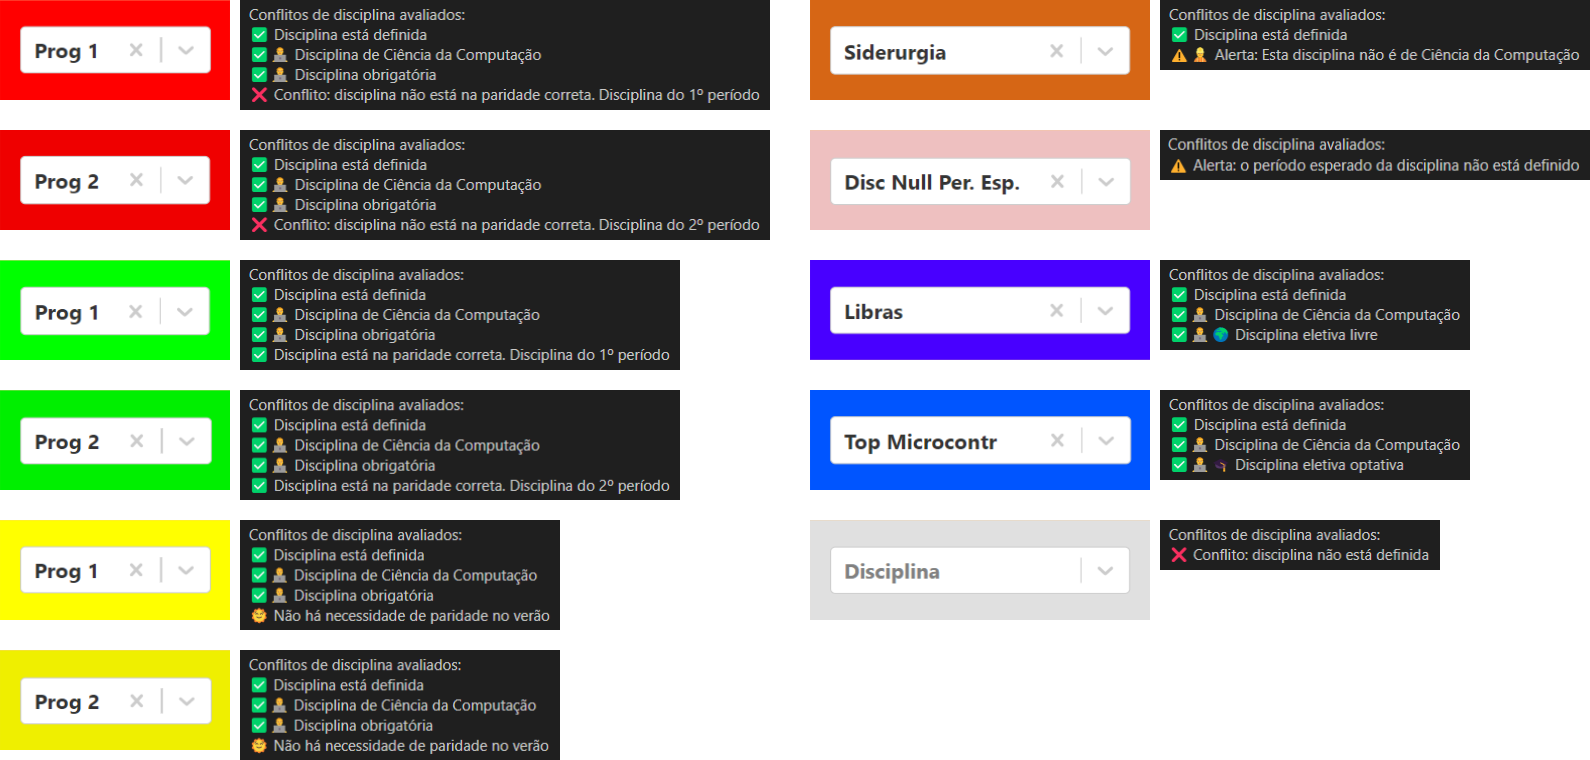
\includegraphics[width=\textwidth]{files/img/Codificacao/Conflitos/Categorias Disciplinas}
\end{MyCenteredFigure}

Já no lado esquerdo da \autoref{fig:conflitoDisciplinaTitulos}, vemos os conflitos que correlacionam os períodos esperados das disciplinas obrigatórias do curso de Ciência da Computação com o semestre em que foram ofertadas. Os semestres possíveis são três: o primeiro semestre, o segundo semestre e o ``período de verão''. No caso do período de verão, as disciplinas que têm o seu período esperado neste semestre são marcadas com um tom amarelado, visto que não há relevância da sua paridade em um período de férias. Já nos casos das disciplinas de paridade ímpar (disciplinas dos períodos 1, 3, 5, 7 e 9) no primeiro semestre, ou as disciplinas de paridade par (disciplinas dos períodos 2, 4, 6, 8 e 10) no segundo semestre, estas são marcadas com um tom esverdeado, sendo aquelas referentes aos períodos finais do curso marcadas com um tom mais escuro. Já as disciplinas pares em semestres ímpares, ou as disciplinas ímpares em semestre pares, são ilustradas com a cor avermelhada, seguindo a mesma lógica de gradiente escuro nos últimos períodos.
